% mnras_template.tex 
%
% LaTeX template for creating an MNRAS paper
%
% v3.0 released 14 May 2015
% (version numbers match those of mnras.cls)
%
% Copyright (C) Royal Astronomical Society 2015
% Authors:
% Keith T. Smith (Royal Astronomical Society)

% Change log
%
% v3.0 May 2015
%    Renamed to match the new package name
%    Version number matches mnras.cls
%    A few minor tweaks to wording
% v1.0 September 2013
%    Beta testing only - never publicly released
%    First version: a simple (ish) template for creating an MNRAS paper

%%%%%%%%%%%%%%%%%%%%%%%%%%%%%%%%%%%%%%%%%%%%%%%%%%
% Basic setup. Most papers should leave these options alone.
\documentclass[fleqn,usenatbib]{mnras}

% MNRAS is set in Times font. If you don't have this installed (most LaTeX
% installations will be fine) or prefer the old Computer Modern fonts, comment
% out the following line
\usepackage{newtxtext,newtxmath}
% Depending on your LaTeX fonts installation, you might get better results with one of these:
%\usepackage{mathptmx}
%\usepackage{txfonts}

% Use vector fonts, so it zooms properly in on-screen viewing software
% Don't change these lines unless you know what you are doing
\usepackage[T1]{fontenc}
\usepackage{ae,aecompl}


%%%%% AUTHORS - PLACE YOUR OWN PACKAGES HERE %%%%%

% Only include extra packages if you really need them. Common packages are:
\usepackage{graphicx}	% Including figure files
\usepackage{amsmath}	% Advanced maths commands
\usepackage{amssymb}	% Extra maths symbols

%%%%%%%%%%%%%%%%%%%%%%%%%%%%%%%%%%%%%%%%%%%%%%%%%%

%%%%% AUTHORS - PLACE YOUR OWN COMMANDS HERE %%%%%

% Please keep new commands to a minimum, and use \newcommand not \def to avoid
% overwriting existing commands. Example:
%\newcommand{\pcm}{\,cm$^{-2}$}	% per cm-squared

\usepackage{verbatim}   % added by JP for the TC word count output.

%%%%%%%%%%%%%%%%%%%%%%%%%%%%%%%%%%%%%%%%%%%%%%%%%%

%%%%%%%%%%%%%%%%%%% TITLE PAGE %%%%%%%%%%%%%%%%%%%

% Title of the paper, and the short title which is used in the headers.
% Keep the title short and informative.
\title[Radon trace profiles of PSB galaxies]{MNRAS \LaTeXe\ template -- title goes here}

% The list of authors, and the short list which is used in the headers.
% If you need two or more lines of authors, add an extra line using \newauthor
\author[J. Proctor et al.]{
John Proctor,$^{1,2}$\thanks{E-mail: jp210@st-andrews.ac.uk (JP)}
% A. N. Other,$^{2}$
% Third Author$^{2,3}$
% and Fourth Author$^{3}$
\\
% List of institutions
$^{1}$Royal Astronomical Society, Burlington House, Piccadilly, London W1J 0BQ, UK\\
$^{2}$School of Physics and Astronomy, University of St Andrews, North Haugh, St Andrews KY16 9SS, UK\\
}


% These dates will be filled out by the publisher
\date{Accepted XXX. Received YYY; in original form ZZZ}

% Enter the current year, for the copyright statements etc.
\pubyear{2019}

% Don't change these lines
\begin{document}
\label{firstpage}
\pagerange{\pageref{firstpage}--\pageref{lastpage}}
\maketitle

% Abstract of the paper
\begin{abstract}
A short document to present and discuss Radon trace profiles of stellar velocity maps for a sample of 30 central-type post-starburst galaxies. 
\end{abstract}

% Select between one and six entries from the list of approved keywords.
% Don't make up new ones.
\begin{keywords}
keyword1 -- keyword2 -- keyword3
\end{keywords}

%%%%%%%%%%%%%%%%%%%%%%%%%%%%%%%%%%%%%%%%%%%%%%%%%%

%%%%%%%%%%%%%%%%% BODY OF PAPER %%%%%%%%%%%%%%%%%%

\section{Introduction}

This is a simple template for authors to write new MNRAS papers.
See \texttt{mnras\_sample.tex} for a more complex example, and \texttt{mnras\_guide.tex}
for a full user guide.

All papers should start with an Introduction section, which sets the work
in context, cites relevant earlier studies in the field by \citet{Others2013},
and describes the problem the authors aim to solve \citep[e.g.][]{Author2012}.

Testing citations in the bibliography file see e.g. \citet{2019ApJ...872...76N}.

\section{Methods, Observations, Simulations etc.}

Normally the next section describes the techniques the authors used.

\section{Radon trace plots}
\label{Radon-trace-plots}

\begin{figure*}
    \centering
    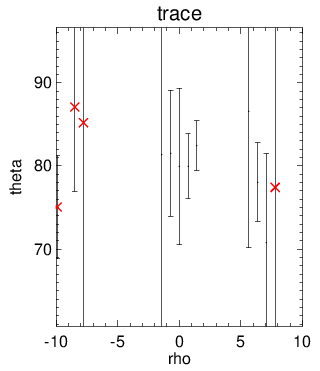
\includegraphics[width=0.19\textwidth]{Images/trace-plots/trace-plots-cpsbs/7964-1902.png}
    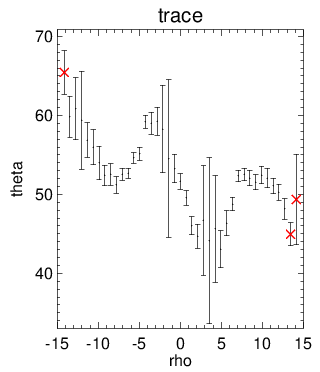
\includegraphics[width=0.19\textwidth]{Images/trace-plots/trace-plots-cpsbs/8080-3702.png}
    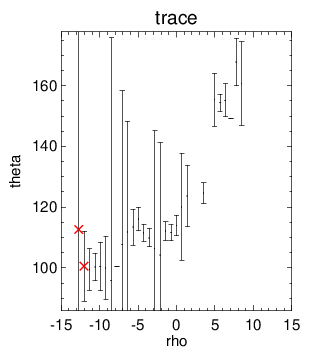
\includegraphics[width=0.19\textwidth]{Images/trace-plots/trace-plots-cpsbs/8081-3702.png}
    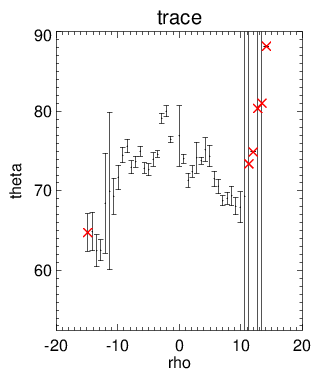
\includegraphics[width=0.19\textwidth]{Images/trace-plots/trace-plots-cpsbs/8082-3704.png}
    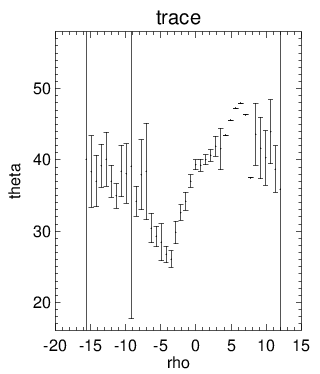
\includegraphics[width=0.19\textwidth]{Images/trace-plots/trace-plots-cpsbs/8143-3703.png}
    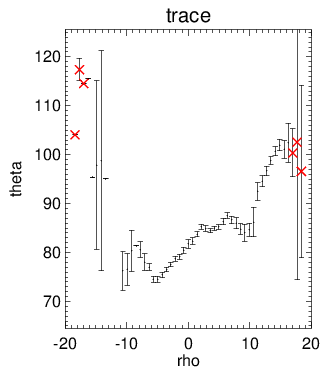
\includegraphics[width=0.19\textwidth]{Images/trace-plots/trace-plots-cpsbs/8313-6101.png}
    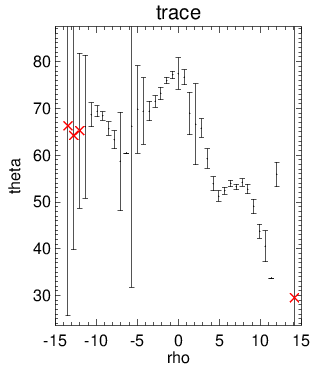
\includegraphics[width=0.19\textwidth]{Images/trace-plots/trace-plots-cpsbs/8315-3703.png}
    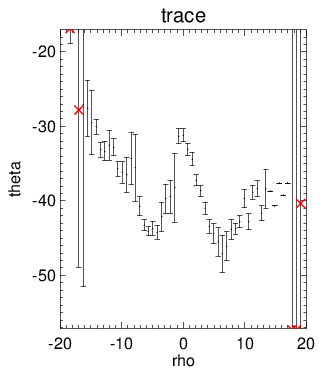
\includegraphics[width=0.19\textwidth]{Images/trace-plots/trace-plots-cpsbs/8331-6104.png}
     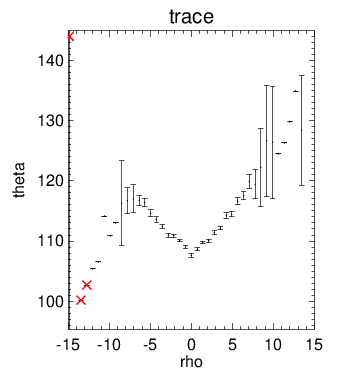
\includegraphics[width=0.19\textwidth]{Images/trace-plots/trace-plots-cpsbs/8555-3701.png}
    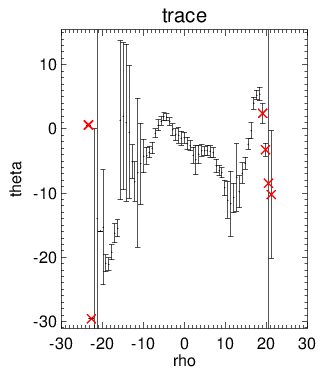
\includegraphics[width=0.19\textwidth]{Images/trace-plots/trace-plots-cpsbs/8623-9102.png}
    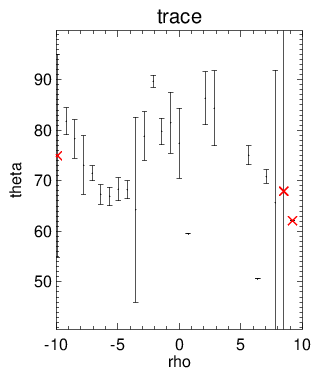
\includegraphics[width=0.19\textwidth]{Images/trace-plots/trace-plots-cpsbs/8655-1902.png}
    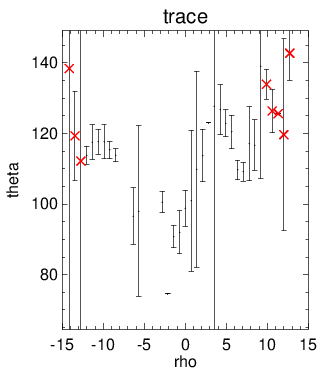
\includegraphics[width=0.19\textwidth]{Images/trace-plots/trace-plots-cpsbs/8713-3701.png}
    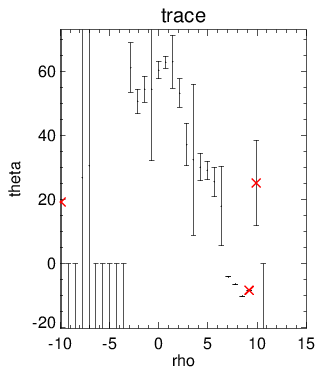
\includegraphics[width=0.19\textwidth]{Images/trace-plots/trace-plots-cpsbs/8725-1902.png}
    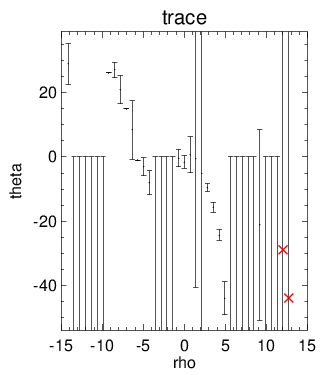
\includegraphics[width=0.19\textwidth]{Images/trace-plots/trace-plots-cpsbs/8933-3704.png}
    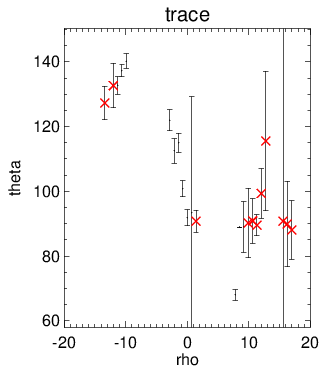
\includegraphics[width=0.19\textwidth]{Images/trace-plots/trace-plots-cpsbs/8934-9101.png}
    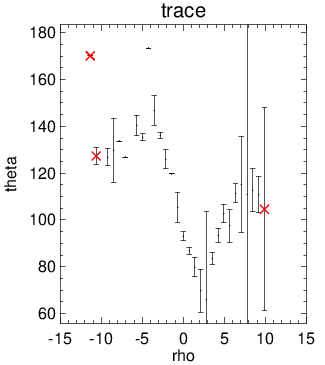
\includegraphics[width=0.19\textwidth]{Images/trace-plots/trace-plots-cpsbs/8935-12701.png}
    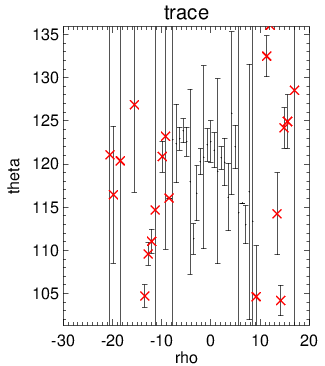
\includegraphics[width=0.19\textwidth]{Images/trace-plots/trace-plots-cpsbs/8938-6102.png}
    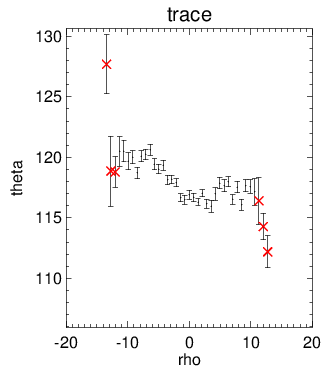
\includegraphics[width=0.19\textwidth]{Images/trace-plots/trace-plots-cpsbs/8941-3701.png}
    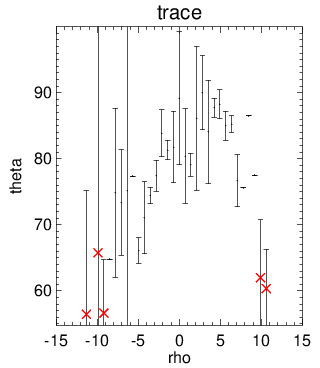
\includegraphics[width=0.19\textwidth]{Images/trace-plots/trace-plots-cpsbs/8944-1902.png}
    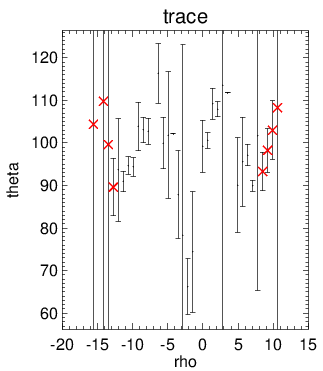
\includegraphics[width=0.19\textwidth]{Images/trace-plots/trace-plots-cpsbs/8950-3704.png}
    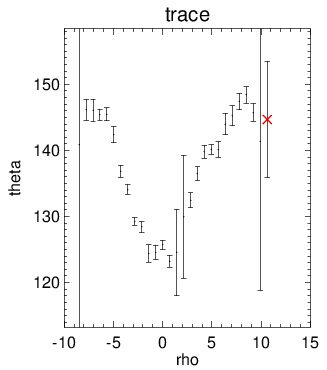
\includegraphics[width=0.19\textwidth]{Images/trace-plots/trace-plots-cpsbs/8979-1902.png}
    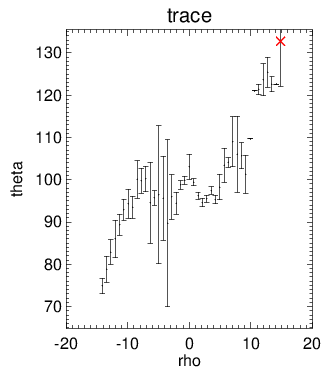
\includegraphics[width=0.19\textwidth]{Images/trace-plots/trace-plots-cpsbs/8996-3704.png}
    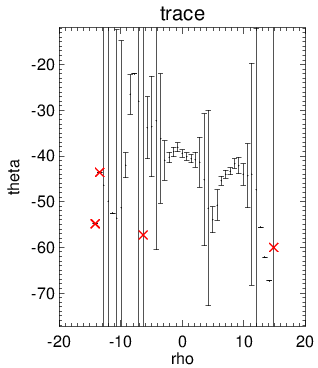
\includegraphics[width=0.19\textwidth]{Images/trace-plots/trace-plots-cpsbs/8997-3704.png}
    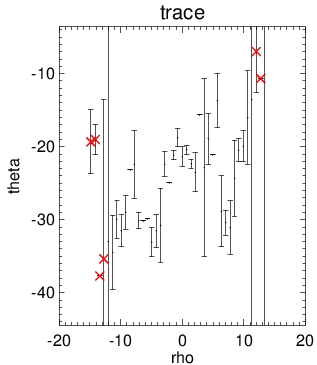
\includegraphics[width=0.19\textwidth]{Images/trace-plots/trace-plots-cpsbs/9047-3701.png}
    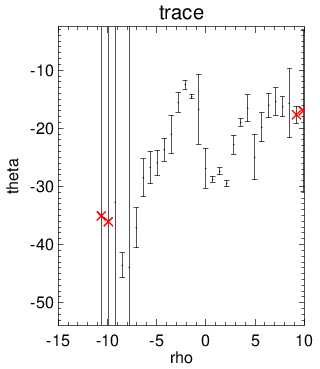
\includegraphics[width=0.19\textwidth]{Images/trace-plots/trace-plots-cpsbs/9085-1902.png}
    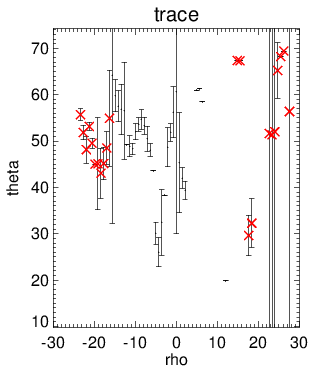
\includegraphics[width=0.19\textwidth]{Images/trace-plots/trace-plots-cpsbs/9493-12705.png}
    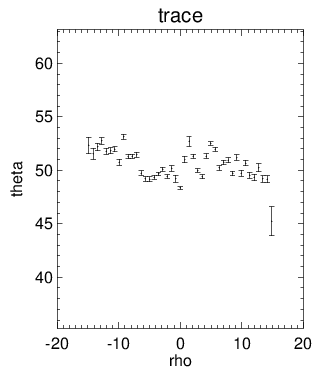
\includegraphics[width=0.19\textwidth]{Images/trace-plots/trace-plots-cpsbs/9494-3701.png}
    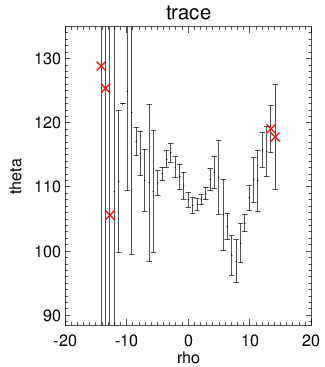
\includegraphics[width=0.19\textwidth]{Images/trace-plots/trace-plots-cpsbs/9494-3703.png}
    \caption{Radon transform trace profiles of the stellar velocity fields of CPSBs with MaNGA plateifu designations as follows. Top row: 7964-1902, 8080-3702, 8081-3702, 8082-3704, 8143-3703; second row: 8313-6101, 8315-3703, 8331-6104, 8555-3701, 8623-9102; third row: 8655-1902, 8713-3701, 8725-1902, 8933-3704, 8934-9101; fourth row: 8935-12701, 8938-6102, 8941-3701, 8944-1902, 8950-3704; fifth row: 8979-1902, 8996-3704, 8997-3704, 9047-3701, 9085-1902; bottom row: 9493-12705, 9494-3701, 9494-3703.}
    \label{fig:Radon-traces-CPSBs}
\end{figure*}



\section{Conclusions}

The last numbered section should briefly summarise what has been done, and describe the final conclusions which the authors draw from their work.

\section*{Acknowledgements}

The Acknowledgements section is not numbered. Here you can thank helpful colleagues, acknowledge funding agencies, telescopes and facilities used etc.
Try to keep it short.

%%%%%%%%%%%%%%%%%%%%%%%%%%%%%%%%%%%%%%%%%%%%%%%%%%

%%%%%%%%%%%%%%%%%%%% REFERENCES %%%%%%%%%%%%%%%%%%

% The best way to enter references is to use BibTeX:

\bibliographystyle{mnras}
\bibliography{JPbib2019} % if your bibtex file is called example.bib

% Alternatively you could enter them by hand, like this:
% This method is tedious and prone to error if you have lots of references
\begin{thebibliography}{99}
\bibitem[\protect\citeauthoryear{Author}{2012}]{Author2012}
Author A.~N., 2013, Journal of Improbable Astronomy, 1, 1
\bibitem[\protect\citeauthoryear{Others}{2013}]{Others2013}
Others S., 2012, Journal of Interesting Stuff, 17, 198
\end{thebibliography}

%%%%%%%%%%%%%%%%%%%%%%%%%%%%%%%%%%%%%%%%%%%%%%%%%%

%%%%%%%%%%%%%%%%% APPENDICES %%%%%%%%%%%%%%%%%%%%%

\appendix

\section{Some extra material}

If you want to present additional material which would interrupt the flow of the main paper,
it can be placed in an Appendix which appears after the list of references.

%%%%%%%%%%%%%%%%%%%%%%%%%%%%%%%%%%%%%%%%%%%%%%%%%%


% Don't change these lines
\bsp	% typesetting comment
\label{lastpage}
\end{document}

% End of mnras_template.tex